\documentclass{beamer}

\beamertemplatenavigationsymbolsempty

\mode<presentation>
{
  \usetheme{default}
}

\usepackage[english]{babel}
\usepackage[latin1]{inputenc}
\usepackage{bussproofs}
\usepackage[retainorgcmds]{IEEEtrantools}

% needs debian package texlive-math-extra
\usepackage{stmaryrd} % for \llbracket, \rrbracket

\usepackage{times}
\usepackage[T1]{fontenc}
% Or whatever. Note that the encoding and the font should match. If T1
% does not look nice, try deleting the line with the fontenc.

\usepackage{tikz}
\usetikzlibrary{positioning}
\usetikzlibrary{calc}
\usetikzlibrary{matrix}

\title
{Structural Subtyping for Records}

\author
{Markus~Klinik}

\institute[Radboud University Nijmegen]
{
  Radboud University Nijmegen
}

\date
{Compiler Construction 2013}


\newcommand{\arr}{\rightarrow}
\newcommand{\Arr}{\Rightarrow}
\newcommand{\semantics}[1]{\llbracket #1 \rrbracket}
\newcommand{\semanticsFd}[1]{\semantics{#1}_{F\delta}}

\begin{document}

\begin{frame}
  \titlepage
\end{frame}

\begin{frame}[fragile]{We've All Been There}

\begin{verbatim}
def printXY(a):
  print a.x
  print a.y

class X:
  x = 10

printXY(X())
\end{verbatim}

\end{frame}

\begin{frame}[fragile]{That's What They Want}

\begin{verbatim}
class XY:
  x = []
  y = False

class XYZ:
  x = "Elvis lives"
  y = True
  z = 10

printXY(XY())
printXY(XYZ())
\end{verbatim}

\end{frame}


\begin{frame}{What Is a Record?}

\begin{itemize}
  \item What do we want to do with a record?
  \item Introduction and elimination!
\end{itemize}

\end{frame}


\begin{frame}[fragile]{Introduction And Elimination}

\onslide<+->

Introduction

\begin{verbatim}
var rec = { x=10, y=True }
printXY( { x=10, z=[] } )
\end{verbatim}

\onslide<+->

Elimination

\begin{verbatim}
rec.x
\end{verbatim}

\end{frame}


\begin{frame}[fragile]{But What \emph{is} a Record?}

\onslide<+->

\begin{itemize}
  \item How is it stored in memory?
  \item How does the code for record projection look like?
\end{itemize}

\onslide<+->

The code

\begin{verbatim}
a getX(b b) { return b.x; }
\end{verbatim}

must work for:

\begin{verbatim}
getX({x=10})
getX({y=True,x=False})
\end{verbatim}

and any other combination of fields.

\end{frame}


\begin{frame}[fragile]{Tuples and Lists}

\texttt{(42, True)}

\vspace{3em}

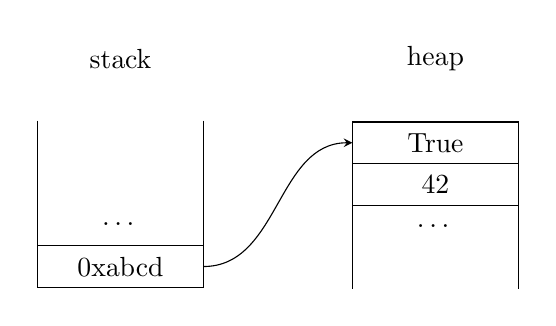
\begin{tikzpicture}

  \matrix (stack) [matrix of nodes
    , nodes={ minimum height = 1.5em
            , minimum width = 6em
            , outer sep = 0pt
            }
    , nodes in empty cells]
  {
    stack \\
    \\
    \\
    \\
    \ldots \\
    |[draw] (address) | 0xabcd \\
  };

  % left and right lines of stack
  \draw (stack-3-1.north west) -- (stack-5-1.south west);
  \draw (stack-3-1.north east) -- (stack-5-1.south east);


  \matrix at (4,0) (heap) [matrix of nodes
    , nodes={ minimum height = 1.5em
            , minimum width = 6em
            , outer sep = 0pt
            }
    , nodes in empty cells]
  {
    heap \\
    \\
    |[draw] (true)| True \\
    |(42)| 42 \\
    \ldots \\
    \\
  };

  % bottom line of cell "42"
  \draw (42.south west) -- (42.south east);

  % left and right lines of heap
  \draw (true.north west) -- (heap-6-1.south west);
  \draw (true.north east) -- (heap-6-1.south east);

  \draw [>=stealth,->] (address.east) to [out=0,in=180] (true.west);

\end{tikzpicture}

\end{frame}

\begin{frame}[fragile]{The shortest crashing C program}

\pause % don't show the first item from the beginning
\begin{itemize}[<+->]
  \item \texttt{main;}
  \item \texttt{int main = 0;}
  \item \texttt{Int main = 0;}
\end{itemize}

\end{frame}

\end{document}
